%%% template.tex
%%%
%%% This LaTeX source document can be used as the basis for your technical
%%% paper or abstract.

%%% The parameter to the ``documentclass'' command is very important.
%%% - use ``review'' for content submitted for review.
%%% - use ``preprint'' for accepted content you are making available.
%%% - use ``tog'' for technical papers accepted to the TOG journal and
%%%   for presentation at the SIGGRAPH or SIGGRAPH Asia conference.
%%% - use ``conference'' for final content accepted to a sponsored event
%%%   (hint: If you don't know, you should use ``conference.'')

\documentclass[tog]{acmsiggraph}

\usepackage{wrapfig}

%%% Make the ``BibTeX'' word pretty...

\def\BibTeX{{\rm B\kern-.05em{\sc i\kern-.025em b}\kern-.08em
    T\kern-.1667em\lower.7ex\hbox{E}\kern-.125emX}}

%%% Used by the ``review'' variation; the online ID will be printed on 
%%% every page of the content.

\TOGonlineid{45678}

%%% Used by the ``preprint'' variation.

\TOGvolume{0}
\TOGnumber{0}

\title{Perceptual Propagation - Episode VI: \\ Return of the Psychoacoustic Kick-Ass}

\author{Chris Malloy and Aidos Abzhanov\\University of North Carolina at Chapel Hill}
\pdfauthor{}

\keywords{sound propagation, perceptual importance sampling}

\begin{document}

%%% This is the ``teaser'' command, which puts an figure, centered, below 
%%% the title and author information, and above the body of the content.

 \teaser{
   \includegraphics[height=1.5in]{figs/teaser}
   \caption{The System Design.}
 }

\maketitle

\begin{abstract}

We introduce a new method for optimizing the performance of path-based sound propagation phase of 3D audio simulation system by leveraging the perceptual feedback from the auralization (and rendering) stage. Our method combines using of psychoacoustics measures to prioritize perceptually important paths and guiding the ray tracing algorithm to better distribute rays to sources ...

% Exploit perceptual limitations of the human auditory system. Compression due to removal of perceptually irrelevant part of the signal. Results in inaudiable distortion.

% The human auditory system's inability to to hear quantization noise under condition of auditory masking.


\end{abstract}

\begin{CRcatlist}
  \CRcat{I.3.5}{Computer Graphics}{Computational Geometry and Object Modeling}{Physically based modeling}
  \CRcat{I.3.5}{Computer Graphics}{Applications}{Sound rendering};
\end{CRcatlist}

\keywordlist

%% Required for all content. 

\copyrightspace


\section{Introduction}
[intro]

Need to cover:
\begin{itemize}
\item The goal of the project
\item prior work
\item results 
\item list of open issues 
\end{itemize}

GSound in \cite{schissler2011gsound}, and \cite{schissler2014high}. Review of perceptual coding \cite{painter2000perceptual}. 


\newpage
\section{Related Work}
GSound in \cite{schissler2011gsound}, and \cite{schissler2014high}. Review of perceptual coding \cite{painter2000perceptual}. 

\section{Introduction to Psychoacoustics}
%\paragraph{Intro}
Psychoacoustics is the science of auditory perception and the human experience of hearing.
Limitations induced by the psychological and physiological mechanisms responsible for hearing are of particular 
interest and have been successfully applied to musical composition, architecture, digital audio coding, and mixing/rendering 
sound.
%and in particular the limitations induced by the psychological and physiological
%mechanisms responsible for the experience of hearing.
Individual psychoacoustic effects and illusions are refered to as \emph{psychoacoustic principles} and include:

\begin{itemize}
\item The Absolute Threshold of Hearing
\item Critical Band Frequency Analysis
\item Simultaneous Masking
\item Non-Simultaneous Masking
\item The Spread of Masking
\end{itemize}

In this method we seek to demonstrate how these basic psychoacoustic principles can be leveraged in a geometric sound propagation 
pipeline, with our most novel contribution being the use of masking in the propagation phase of sound simulation.

\paragraph{Auditory Filters and the Bark Scale of Critical Bandwidths}
%The frequency of sound is conventionally measured in hertz but alternative scales based on human perception are more commonly used
%in psychoacoustic literature and models.
%These include the Bark and ERB frequency scales, both of which are based on the frequency resolution of human hearing and are derived 
%from listening experiments.
%Although sound frequency is conventionally measured in hertz, for the purpose of psychoacoustic modelling it is preferable to use a 
%scale based on the frequency resolution of human hearing.
%The most common scale used in psychoacoustic literature is the Bark scale, which has units directly proportional to the frequency-dependent 
%bandwidth at which individual tones can be perceived separately.
%The Bark scale is measured in \textbf{critical bands}, 
%Frequency scales based on the resolution of human hearing are used for modelling psychoacoustic principles, most commonly the Bark scale.
%The Bark scale is measured in units of \emph{critical bands}

The perception of sound frequency is mediated by the \textbf{basilar membrane}, a coiled structure of the inner ear that vibrates in response 
to sound energy.
Regions of the basilar membrane have a characteristic frequency they are most sensitive to. This characteristic frequency is highest at the 
base of the basilar membrane and continuously decreases along it's length.
\paragraph{}
Pure tones result in patterns of excitation on the basilar membrane that may overlap for sounds that are nearby in frequency, and for this reason the 
basilar membrane is abstracted in literature as a bank of overlapping \textbf{auditory filters}.
%The bandwidth of an auditory filter is referred to as it's \textbf{critical bandwidth}
\textbf{The Bark frequency scale} is measured in units of the frequency-dependent bandwidths of the auditory filters of the basilar membrane, refered 
to as the \textbf{critical bandwidths}, and is a commonly used frequency scale in psychoacoustics because it is directly proportional to the frequency 
resolution of human hearing.
%whose bandwidths are measured by \textbf{the Bark scale}.
%Both the Bark scale and the curves representing auditory filters along the basilar membrane have been derived from listening experiments.
%The shape of these auditory filters have been derived from listening experiments and used to design a frequency scale proportional to the 
%frequency resolution of human hearing
%, and this overlap 
%has been measured through listening experiments.
\paragraph{Spectral Masking}
\begin{figure}
  \centerline{\includegraphics[width=2.8in]{figs/bmem}}
  \caption{The basilar membrane}
  \label{fig:basilarmembrane}
\end{figure}

\begin{figure}
  \centerline{\includegraphics[width=2.8in]{figs/auditoryfilters}}
  \caption{Curves representing the response of auditory filters as a function of center frequency}
  \label{fig:auditoryfilters}
\end{figure}
Because of the observed overlap of auditory filters, a loud tone will also excite regions of the basilar membrane
that should correspond to neighboring frequencies. 
This interference of excitation is the phenomenon of \textbf{spectral masking}, where a tone played at a given 
frequency will perceptually occlude relatively softer tones that are nearby in frequency.
The intensity of masking is assymetric in frequency with lower tones masking higher tones with a higher intensity
than the reverse.
This psychoacoustic principle has been referred to as \textbf{the upward spread of masking} (the axis of `upward' being frequency).
\paragraph{}
\begin{figure}
  \centerline{\includegraphics[width=2.8in]{figs/masked}}
  \caption{Absolute threshold of hearing and masked threshold}
  \label{fig:masked}
\end{figure}
The \textbf{absolute threshold of hearing} is a curve of minimum pressure level necessary to perceive a sound at 
a given frequency and in the presence of relative quiet.
Similarly, a \textbf{masking threshold} characterizes the threshold below which a sound is made imperceptible
in the presence of a masker.
The net result of spectral masking in the presence of multiple tones is approximately additive, and the net amount of 
masking continues to effect later tones after the masking tone has ended because of a phenomenon referred to as \textbf{non-simultaneous} or \textbf{temporal masking}.

%The basilar membrane is the auditory equivalent of the human eyes.
%It mediates human auditory perception as well as the phenomenon of spectral masking.
%The following is a brief overview of it's function as it relates to psychoacoustic principles.


\section{MPEG Psychoacoustic Models}
The MPEG-1 audio standard specifies an algorithm for compressing digital audio signals by removing the perceptually inaudible components. The standard defines two psychoacoustic models that model the human sound perception system and inform the quantization of individual audio blocks during compression. The models differ in computational complexity, but share the main idea of splitting sound into tone-masking-noise and noise-masking-tone, and calculating a global masking threshold curve  by combining the two individual models based on how tonal or noise-like the signal is. This global masking threshold represents the minimal sound power perceptible by the average human listener. The global threshold guides the encoders allocation of bits to better represent an error-free signal. In the psychoacoustic model 1 the tonality of a component is determined from peaks in the critical bands, while in the model 2, it is determined using a predictability measure.
 
 The psychoacoustic models involve following main steps of the global masking threshold computation:
 \begin{itemize}
 \item Spectral Analysis: calculation of the \emph{power spectral density} (PSD) which describes the distribution of the power of a signal over the different frequencies.
 \item Critical Band Analysis: the power spectrum of the signal is partitioned into critical bands by integrating over the corresponding bandwidths.
 \item Tonality Analysis: the \emph{spectral flatness measure} (SFM) is used to characterize the spectrum of the signal. The SFM is defined as the ratio of the geometric to arithmetic mean values of power spectral density. The \emph{tonality index} (TI) is calculated by comparing estimated SFM with the SFM of a sinusoidal signal. Values of the tonality index that are closer to zero indicate that the spectrum of the signal look similar to a spectrum of white noise. Values of TI that are closer to one indicate that the spectral power is concentrated in a relatively small number of bands and the signal sounds like a mixture of sine waves.
 \item Masking Analysis: The masking threshold is determined by calculating an offset to the excitation pattern. Due to asymmetry of tone and noise maskings the value of offset depends on the value of the tonality index. The final values for the offset are interpolated from the offsets for tone-like and noise-like signals.
 \item Spread of Masking: Inter-band masking is taken into account by convolving each of the maskers with the \emph{spreading function}.
 \end{itemize}


\section{Overview}

\subsection{Spectral Masking}
Masking thresholds are obtained by performing critical band analysis (with spreading), making a determination of the noise-like or tone-like nature of the signal, applying thresholding rules for the signal quality, then accounting for the absolute hearing threshold \cite{painter2000perceptual}. 
We assume that the input sound samples are given in advance, and can be pre-processed to extract spectral information about the signal. N samples long Hann window with 50 percent overlap is used to produce the parts of the input sound signal that are processed by psychoacoustic module.
% Short time Fourier transform.

The short time spectrum \( X(\omega) \) is computed from the windowed signal chunk \( x(i) \;\; i \in [0, N-1]\) using discrete Fourier transform. From this we generate the \emph{power density spectrum} by
\[ P(\omega) = Re(X(\omega))^2 + Im(X(\omega))^2, \;\; \omega \in [0, N-1]. \]
Signal power for each critical band \(i\) is calculated by summing corresponding power density spectra within that frequency band
\[ B_i = \sum_{\omega = \omega_{i\_low}}^{\omega_{i\_high}} P(\omega). \]
To account for spreading of masking the critical band signal power is convolved 
\[ C_i = B_i * SF_i \]
with the \emph{spreading function} \( SF_i, \) representing masking across critical bands and given by analytical expression:
\[ SF_i = 15.81 + 7.5(\delta i + 0.474) - 17.5\sqrt{1 + (\delta i + 0.474)^2} .\]
Due to the asymmetry of masking there are two masking thresholds: for tone masking noise the threshold is estimated as \( 14.5 + i\) dB below \( C_i \), while for noise masking tone it is estimated as \( 5.5 \) dB below \( C_i \), for each band \( i \). 

In order to recognize a tonal or noise-like signal within a certain number of samples, the \emph{spectral flatness measure} (SFM) is estimated
\[ SFM_{dB} = 10 \log_{10} \frac{\mu_g}{\mu_a}, \]
where \( \mu_g \) and \( \mu_a \) are geometric and arithmetic means of the \( C_i \).

The SFM is compared with the SFM of a sinusoidal signal (entirely tonelike signal with SFM = -60 dB)
and the \emph{tonality index} is calculated \cite{johnston1988estimation} by
\[ \alpha = \min (\frac{SFM_{dB}}{-60}, 1) .\]
SFM = 0 dB corresponds to a noise-like signal and leads to \( \alpha = 0 \), whereas an SFM = 75 dB gives a tone-like signal \( (\alpha = 1) \).

The tonality index is then used to weight the thresholding rules for each band to form an \emph{offset} between signal level and the masking threshold in critical band \( i \)
\[ O_i = \alpha(14.5 + i) + (1 - \alpha)5.5 \;\;\; \text{(in dB)}.\]

Finally, the masking thresholds in the frequency power domain are then formed by subtracting the offsets from the Bark spectral components
\[ T_i = 10^{\log_{10}(C_i) - (O_i/10)} .\]


\subsection{GSound}
\input{gsound.tex



\section{Implementation}
\begin{figure}
  \centerline{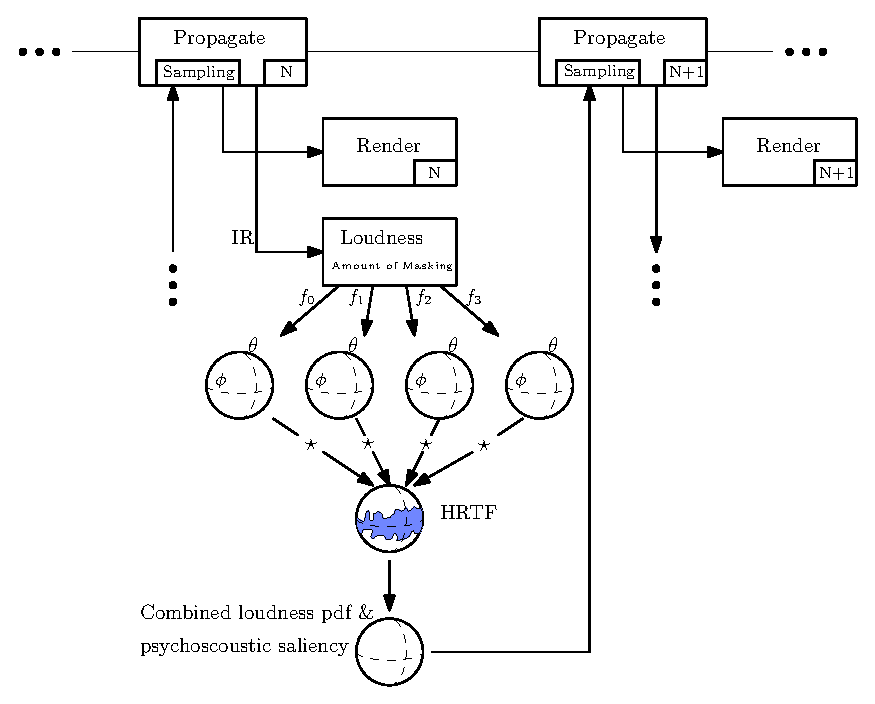
\includegraphics[width=3.0in]{figs/figure1}}
  \caption{Our pipeline}
  \label{fig:figure1}
\end{figure}

The general pipeline of our system consists of a preprocessing step that is performed on source audio
as well as a runtime component that enables feedback from the auralization of IRs computed in one step of 
propagation to accelerate the next step of propagation.
\paragraph{Preprocessing}
Much of the sound processing performed as part of the MPEG Psychoacoustic Model II can be precomputed 
given a clip of audio that will become a source of sound.
We perform a short-time fourier transform of the audio using 512 sample-wide Hanning windows with a 
50\% overlap between neighboring windows.
We store this in an augmented representation of the source's sound buffer that can interpolate between 
windowed spectrograms to arrive at the frequency representation of the audio corresponding to a specific 
path's delay and start time.
Likewise, we also store and interpolate the power spectral density, tonality, and Bark critical bands 
precomputed from this frequency representation.
When the frequency bands that will be used to discretize sound in the impulse response are known, the 
spreading function used in excitation and masking computations as well as the offsets corresponding 
to noise-masking-tone and tone-masking-noise can also be precomputed.
As is also done in the Psychoacoustic Model II and the work of Nikolas et al, we assume a negligable 
effect due to noise-masking-noise and that the global masking threshold is adequately characterized 
by only the former two.
\paragraph{Perceptual Salience}
Given an impulse response corresponding to propagation step $n$ of the simulation, we compute a measure 
of perceptual salience based on the directionality of loudness and the amount of masking between sampled 
paths that are nearby in time and frequency.
We assume temporal locality of the IR and use this measure of salience as prior knowledge to accelerate 
step $n+1$ of the propagation system.
\paragraph{}
%The computation of perceptual salience involves directional functions that we must represent using a 
%spherical mapping onto a grid of values and rasterize discrete samples onto.
%These spherical functions will ultimately be used for the construction of a probability density function
%of the chance a direction will be samp
For each path of an IR from propagation step $n$, we use it's associated delay to retrieve the precomputed tonality
and power spectral density of the source's sound at that time.
We then compute it's excitation pattern by convolving the precomputed spreading function with the path's power 
spectral density and frequency-binned response.
We also compute for each path it's contribution to the masking threshold of hearing by combining the tone-masking-noise and noise-masking-tone models based on tonality of the signal and store this as an array
of frequency binned thresholds sampled in time.
\paragraph{}
We assume the perceptual salience of a direction from the listener is proportional to the excitation from that direction
above the masking threshold.
We therefore compute our measure of salience as the amount of excitation from that direction above 
the corresponding threshold associated with the path's delay.
The salience of each path is then rasterized onto a spherical mapping of a grid representing directions about the 
listener. 
Because we are sampling discrete, possibly sparse, paths onto a spherical function that will ultimately be used as a 
a probability density function, we rasterize the path's salience onto the sphere using a gaussian kernel 
instead of the nearest cell (as is done in kernel density estimation).
\paragraph{Path Sampling}
Paths at propagation step $n+1$ are sampled around the listener by Monte-Carlo sampling of the 
spherical salience function generated from the IR of propagation step $n$.
The probability of sampling a path from a given direction becomes proportional to the normalized 
salience in that direction and the path's sound power is then inversely scaled by the normalized 
salience as a bias correction.
As a result, paths that are perceptually negligible in their contribution to the final rendered audio 
will be sampled less often and fewer paths will be needed to converge to an accurate IR of the scene.
\paragraph{gSound}
In our gSound implementation, we perform the per-sound precomputation as the scene is loaded and combine our 
representation with that of the sound buffers and sources.
This accounts for the bulk of processing, the remainder of which is handled per-IR.
For the runtime component we have inserted our system as a separate IR update job running in the same threadpool
as the main system that is executed for each freshly computed IR.
The current salience measure is used in propagation as the next is computed from the most recent IR and is accessible 
for visualization through the main propagation system.
\paragraph{}
Both the sampled and discrete path IR are used to compute salience, and so potentially numerous samples might be 
rasterized to the sphere as a result.
We therefore perform the kernel density estimation of spherical functions by rasterizing each discrete sample to it's 
nearest cell and performing several box filters to approximate a gaussian kernel as a post-processing step.
This approach is much more efficient than rasterizing individual gaussian functions and produces similar results.
In order to avoid distortion from box filtering the 2d grid directly, our spherical mapping is a per-hemisphere 
Lambert cylindrical projection.


%\section{Conclusions}
%\input{src/conclusions.tex}

\section{Future Extensions} % instead of limitations and future works
% \paragraph{Limitations}

% \paragraph{Conclusion}

% \paragraph{Future Work}

Evaluate the existing efficiency of the pipeline based on the distribution of paths in the existing renderer.
Conduct user study.

Decouple the propagation to include both backward and forward paths (carrying importance and source information respectively)
% Incorporate bidirectional ray tracing instead of backwards ray tracing of the sound paths.

Try strategies to connect the paths and guide sampling on both ends to converge more efficiently

Improve sampling schemes based on the state-of-the-art algorithms from graphics field.

Binaural masking.

Incorporate the support of temporal masking (forward, backward)

Go deeper into Rendering part of the system (how can we use psychoacoustic principles there)



% \begin{table}[ht]
%   \centering
%   \caption{A simple table.}
%   \begin{tabular}{|r|l|}
%     \hline
%     7C0 & hexadecimal \\
%     3700 & octal \\ \cline{2-2}
%     11111000000 & binary \\
%     \hline \hline
%     1984 & decimal \\
%     \hline
%   \end{tabular}
% \end{table}


% The SIGGRAPH citation format is the ``author year''
% format~\cite{Pellacini:2005:LAH}. The year is separated from the
% author by a single space~\cite{yee:2000:ssa}. Two authors are
% separated by the word ``and''~\cite{parke:1996:CFA}. More than two
% authors are represented by the primary author and ``et al.''~\cite{levoy:2000:TDM}.

% Multiple citations at a single point in the content are separated by
% semicolons~\cite{levoy:2000:TDM,sako:2001:SSB}.

% When the last name of the cited author is part of the text, it may be
% omitted from the citation: ``\ldots as shown in Fedkiw et
% al.~\shortcite{fedkiw:2001:VSO}, the coefficient remains\ldots''


% Shown in Figure~\ref{fig:ferrari}.

% \begin{figure}[ht]
%   \centering
%   \includegraphics[width=3.0in]{images/ferrari_laferrari}
%   \caption{Ferrari LaFerrari. Image courtesy Flickr user ``gfreeman23.''}
%   \label{fig:ferrari}
% \end{figure}

%\section{Contact Information}
%
%If you have questions or suggestions regarding this document, please
%contact us at ``gamma@cs.unc.edu''.

\section*{Acknowledgements}

To Celeste, for the pizza and coffee, and Hasan, for all the bagels.

\bibliographystyle{acmsiggraph}
\nocite{*}
\bibliography{src/references}
\end{document}
